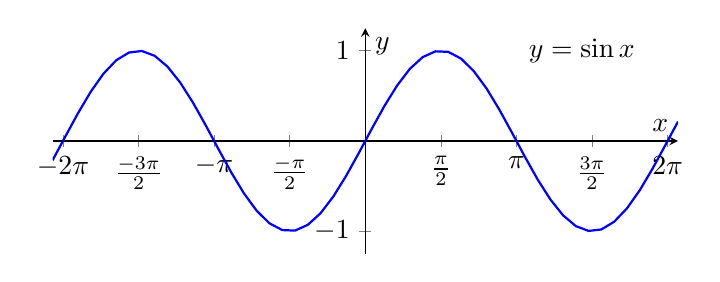
\begin{tikzpicture} 
\begin{axis}[
	width=3.75in,
	height=1.75in,
	axis lines = middle,
	xmin=-6.5, 
	xmax=6.5, 
	ymin=-1.25, 
	ymax=1.25, 
	xlabel=${x}$,
	ylabel=${y}$,
	xtick={-2*pi,-3*pi/2,-pi,-pi/2,pi/2,pi,3*pi/2,2*pi},
	ytick={-1,1},
	xticklabels = {${-2\pi}$,${\frac{-3\pi}{2}}$,${-\pi}$,${\frac{-\pi}{2}}$,${\frac{\pi}{2}}$,${\pi}$,${\frac{3\pi}{2}}$,${2\pi}$},
]
% defines the function
\addplot[  
	domain=-6.5:6.5, % the domain of the function
	blue, 
	thick,
	samples=50,
]
{sin(deg(x))};

\node at (axis cs:  4.5,1) {${\bm{y=\sin x}}$};


\end{axis}
\end{tikzpicture} 